\section{Data Grouping}
Only grouping the data on vehicles will give too few and too diverse groups of which it will be difficult to make usable conclusions. 
The data therefore needs to be grouped into smaller units.
In the following we will use two different grouping strategies, periods and trips, explained in the sections below.
Figure~\ref{fig:groupings} shows the two concepts.
The top lines indicate three trips where the ``gaps" represent time between two trips.
A trip can thereafter contain smaller periods indicated by the boxes below.
A period is a stretch of time where some property holds, e.g. the vehicle drives at the same speed or the vehicle is idling.

\begin{figure}[htb]
\centering
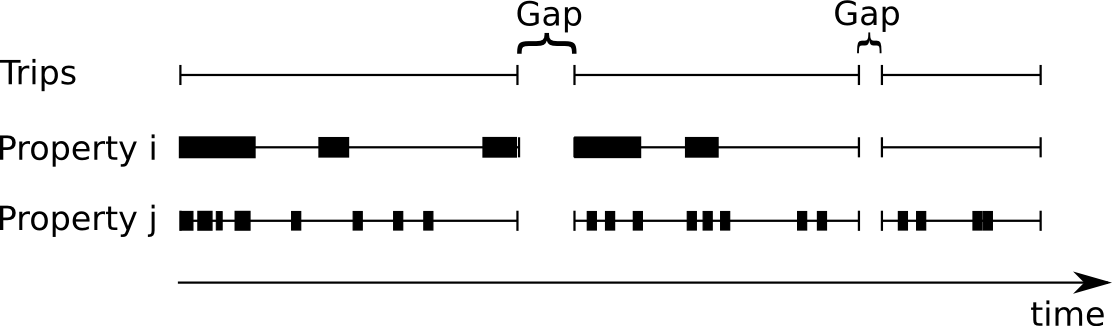
\includegraphics[width=0.45\textwidth]{../images/groupings.png}
\caption{Example of periods and trips}
\label{fig:groupings}
\end{figure}

\subsection{Trips}\label{sec:trips} 
This temporal and sometimes spatial grouping looks primarily on the time difference between trips, the length of the trip and sometimes the location of the vehicle.
The data set is split into trips by annotating each record with a trip identifier, \tid{\rec{}}.
A trip, \trip{} is defined as a consecutive sequence of at least 30 records with the same vehicle identifier where the engine is turned on and any two consecutive records are within 120 seconds.
\begin{align} %TODO: I still do not like this one
\timestamp{\rec{j+1}}-\timestamp{\rec{j}}&< 120\nonumber\\
|\trip{}|&\geq 30\nonumber\\
\tid{\rec{j}}=\tid{\rec{j+1}}&=\tid{\trip{}}\nonumber\\
\vid{\rec{j}}=\vid{\rec{j+1}}\nonumber
\end{align}
where $j$ ranges over the records in the trip.

Idle time, i.e. when the engine is running but the vehicle is not moving (see Section~\ref{sec:idle}), is an important factor for fuel consumption, and we therefore need to ensure that these records are included in the trips. 
A trip is hence defined from when the engine of the vehicles engine is running, that is when $\rpm{\rec{}}> 0$.
In order not to split a trip into two just because the engine stalls, we say that a trips ends when the time cap between two consecutive records is too large.
Figure~\ref{fig:TimeTrips} shows the number of trips when varing the time gap from 5 seconds between two trips to 200 seconds.
We see that the curve flattens around 120 seconds and we choose this as the gap.
Short trips with few records will not give a usable idea of which factors influence fuel consumption.
Figure~\ref{fig:LengthTrips} show the number of trips varying the minimum number of records in a trip.
The curve flattens around 30 records, which in most cases will correspond with 30 seconds. 
A similar test using time as the minimum requirement on trips show no clear result. 
\begin{figure}[htb]
\centering
\includegraphics[width=0.45\textwidth]{../src/d_images/TimeTrips.png}
\caption{Number of trips at different timeframes}
\label{fig:TimeTrips}
\end{figure}
\begin{figure}[htb]
\centering
\includegraphics[width=0.45\textwidth]{../src/d_images/TripsLength.png}
\caption{Number of trips at different lengths}
\label{fig:LengthTrips}
\end{figure}

\subsection{Periods}\label{sec:periods}%TODO: Other name?
It will some times be more interesting to look at records with a similar propery than looking solely at trips.
Let a period be a sequence of consecutive records within a trip with some similar property.
The example in Table~\ref{tb:periods} shows two period groupings on a small sample set.
The property of period X is that the speed is exactly the same as that of the previouse record.
The sample set hence contains 2 periods with this property.
The propery of period Y is that the vehicle is accelerating which results in two different periods.
Let $\timelength{p}$ be the length of period, $p$ in seconds. %TODO: Do we use this?

\begin{table}
\centering
\begin{tabular}{|c|c|c|c|c|}\hline
record id & speed & tid & Period X & Period Y\\\hline
\rec{1} & 59 & 0 &   & a \\\hline
\rec{2} & 60 & 1 & 1 & a\\\hline
\rec{3} & 60 & 1 & 1 &  \\\hline
\rec{4} & 60 & 1 & 1 &  \\\hline
\rec{5} & 63 & 1 &   & b\\\hline
\rec{6} & 64 & 1 &   & b\\\hline
\rec{7} & 67 & 1 & 2 & b\\\hline
\rec{8} & 67 & 1 & 2 &  \\\hline
\rec{9} & 67 & 2 &   &  \\\hline
\end{tabular}
\caption{Example of period grouping}\label{tb:periods}
\end{table}


